
\section{Problema di Ottimizzazione:} In matematica e in informatica, un problema di ottimizzazione è il problema di trovare la migliore soluzione fra tutte le soluzioni fattibili. Sia f: $\mathbb{R}^n \to \mathbb{R}$ e sia S $\subseteq \mathbb{R}^n$; si definisce \textit{problema di ottimizzazione} un problema formulato nel seguente modo: determinare
\begin{equation*}
    min f(x)
\end{equation*}
sapendo
\begin{equation*}
    x \in S 
\end{equation*}
Oppure nel seguente modo: determinare 
\begin{equation*}
    max f(x)
\end{equation*}
sapendo
\begin{equation*}
    x \in S 
\end{equation*}
Chiamiamo \textit{f} funzione obiettivo e S \textit{l'insieme ammissibile}. Se abbiamo un problema di ottimizzazione, abbiamo allora che:
\begin{itemize}
    \item Il problema si dice inammissibile se S = $\varnothing$
    \item Il problema si dice illimitato inferiormente quando, per ogni M $>$ 0 è possibile trovare una x $\in$ S t.c. f(x) $<$ -M, e si dice illimitato superiormente quando, per ogni M $>$ 0 è possibile trovare una x $\in$ S t.c. f(x) $>$ M
    \item Nel caso in cui si debba determinare il minimo di f(x) il problema ammette soluzione ottima se $\exists x^* \in S$ t.c. f(x$^*$) $\leq$ f(x), $\forall x \in S$. In questo caso chiamiamo $x^*$ minimo globale o soluzione ottima e f(x$^*$) il valore ottimo. Nel caso in cui si debba determinare il massimo di f(x) il problema ammette soluzione ottima se $\exists x^* \in S$ t.c. f(x$^*$) $\geq$ f(x), $\forall x \in S$. Anche in questo caso chiamiamo $x^*$ soluzione ottima e f(x$^*$) il valore della soluzione ottima.
\end{itemize}
Nella trattazione teorica dei problemi di ottimizzazione, per semplicità, decidiamo di scrivere in una sola forma tra min e max. \textit{Per convenzione scegliamo min}:
\begin{equation*}
    min f(x)
\end{equation*}
Anche perché passare dall'una all'altra forma è facilissimo, basta ricordarsi che trovare il min di f(x) equivale a trovare il max di - f(x). Quindi si può passare da un problema di minimo a uno di massimo semplicemente cambiando la funzione.



\subsection{Classificazione dei Problemi:} 
\begin{itemize}
    \item Ottimizzazione continua: quando le variabili possono assumere valori reali
    \begin{itemize}
        \item vincolata quando S $\subset \mathbb{R}^n$
        \item non vincolata quando S = $\mathbb{R}^n$
    \end{itemize}
    \item Ottimizzazione discreta: quando le variabili possono assumere valori interi
    \begin{itemize}
        \item programmazione a numeri interi quando S $\subset \mathbb{Z}^n$
        \item programmazione combinatoria (o programmazione 0/1, o programmazione binaria) quando S $\subseteq \{0,1\}^n$. Molti problemi sono di questo tipo.
        \item programmazione mista-intera quando solo alcune variabili devono assumere valori interi
    \end{itemize}
\end{itemize}
Ora parliamo dell'insieme ammissibile S, esso \underline{solitamente} è descritto da un sistema finito di disuguaglianze del tipo g(x) $\geq$ b (o anche uguaglianze, essendo un'uguaglianza una coppia di disuguaglianze), che chiamiamo \textit{vincoli}, con g(x): $\mathbb{R}^n$ $\to$ $\mathbb{R}$. Cioè:
\begin{equation*}
    S = \{x \in \mathbb{R}^n: g_1(x) \geq b_1, ..., g_m(x) \geq b_m\}
\end{equation*}
Diciamo che, dato un punto $\bar{x}$, un vincolo $g_i(\bar{x}) \geq b_i$ è:
\begin{itemize}
    \item Soddisfatto in $\bar{x}$ quando $g_i(\bar{x}) \geq b_i$ è vera. Un caso particolare è il vincolo attivo, cioè $\bar{x}$ quando $g_i(\bar{x}) = b_i$. Qui il vincolo è soddisfatto ma all'uguaglianza.
    \item Violato in $\bar{x}$ quando $g_i(\bar{x}) \geq b_i$ è falsa
    \item Ridondante quando la sua eliminazione non muta l'insieme ammissibile. Questo non ha nulla a che fare con la soddisfazione o meno del vincolo: un vincolo ridondante può essere anche un vincolo vietato.
\end{itemize}
Quindi, ricapitolando in un problema di ottimizzazione di questo tipo, abbiamo una funzione obiettivo che vogliamo ottimizzare, ad esempio minimizzare:
\begin{equation*}
    min f(x)
\end{equation*}
E m disuguaglianze da rispettare:
\begin{equation*}
    s.t. \hspace{0.2cm} g_i(x) \geq b \hspace{1.5cm} i = 1, ..., m
\end{equation*}
Quando ciò avviene si parla di un problema di Programmazione Matematica. Precisamente si parla di:
\begin{itemize}
    \item Programmazione Matematica Lineare (PL): quando f(x) e tutte le $g_i(x)$ sono lineari
    \item Programmazione Matematica NonLineare (PNL): quando almeno una tra $g_i(x)$ oppure f(x) sono una funzione nonlineare.
\end{itemize}


\paragraph{Facciamo un esempio:} 
\begin{equation*}
    min f(x) = min 3x_1 + x_2
\end{equation*}
Con $3x_1 + x_2$ funzione obiettivo.
\begin{equation*}
    \begin{cases}
        \text{$x_1^2 + x_2^2 \leq 4$}\\
        \text{$x_1 \geq 0$} 
    \end{cases}
\end{equation*}
Sono i nostri vincoli. Che possiamo scrivere nella forma dell'insieme ammissibile in questo modo:
\begin{equation*}
    S = \{x \in \mathbb{R}^2: x_1^2 + x_2^2 \leq 4, x_1 \geq 0\}
\end{equation*}
Bene, classificare il problema. Allora vediamo, abbiamo un insieme ammissibile definito solo attraverso diseguaglianze, e dobbiamo trovare il minimo di una funzione: siamo di fronte a un problema di Programmazione Matematica. Inoltre vediamo che anche se f(x) è lineare, il primo vincolo presenta una funzione non lineare, quindi è una PLN.

\paragraph{E questo esempio?} 
\begin{equation*}
    min 3x_1 + 4x_1 
\end{equation*}
Con vincoli:
\begin{equation*}
\begin{cases}
    \text{$log(2)x_1 + sin(\pi/3)x_2 \geq 7$}\\
    \text{$x_2 \leq 0$}
\end{cases}
\end{equation*}
Questo è un PL: infatti la funzione obiettivo è lineare, e - non facciamoci ingannare dai coefficienti - anche i vincoli lo sono.

\paragraph{Ultimo esempio...}
\begin{equation*}
    min sin(x_1) + 8x_2
\end{equation*}
Con vincolo:
\begin{equation*}
(x_1,x_2) \in S \Longleftrightarrow x_1 \hspace{0.2cm} \text{è un numero pari} \hspace{0.2cm} \lor \hspace{0.2cm} x_1 = 7^m,  m \in \mathbb{N}
\end{equation*}
Qua vediamo che i vincoli (che in questo caso è uno solo) che formano l'insieme ammissibile non sono tutte disuguaglianze, quindi questo non è un problema di Programmazione Matematica. Ma è comunque un problema di ottimizzazione. Il discorso è che noi, in questo corso, questi tipi di problemi non li considereremo, perché consideriamo solo quelli di Programmazione Matematica e, per la maggior parte del corso, esclusivamente i PL. Vediamo ora un esempio di Programmazione Matematica Binaria.

\subsection{Problema di Capital Budgeting, Programmazione Binaria:} 
Un piccoloinvestitore deve stabilire come investire il proprio capitale potendo
scegliere tra 6 dierenti investimenti. L'investitore dispone di un budget di
100000e e conosce i costi di attivazione nonché il Net Present Value (NPV)
di ciascuno di essi come riportato nella tabella che segue:
\begin{table}[h!]
    \centering
    \begin{tabular}{|c||c|c|}
    \hline
    & costo (in migliaia di \euro) & NPV\\
    \hline
    \hline
    inv.1 & 100 & 40\\
    \hline
    inv.2 & 50 & 35\\
    \hline
    inv.3 & 45 & 18\\
    \hline
    inv.4 & 20 & 4\\
    \hline
    inv.5 & 10 & 10\\
    \hline
    inv.6 & 5 & 2\\
    \hline
    \end{tabular}
\end{table}
Quali investimenti attivare per fare in modo che il NPV sia il più grande possibile? Questo è un problema particolare: mentre nel problema precedente dovevamo scegliere quanto produrre, e le soluzioni potevano essere frazionarie, qui le scelte che possiamo fare, per ogni investimento, sono solo 0 o 1 (investimento non attivo o attivo). Per problemi come questo o simili a questo è ragionevole introdurre queste variabili
\begin{equation*}
    x_i = 
    \begin{cases}
        \text{1 se l'investimento i è attivato}\\
        \text{0 altrimenti}
    \end{cases}
\end{equation*}
Quindi avrò un vettore di 6 variabili composto da 0 e 1. Questo viene chiamato \textit{Vettore di Incidenza}, ed è un vettore x $\in$ \{0,1\}$^6$. Quindi siamo di fronte a un problema di Programmazione Matematica binaria. Dato uno di questi vettori, possiamo calcolarci il costo totale degli investimenti scelti dal vettore, così: prendiamo la somma di tutti i costi moltiplicando ognuno di essi per la rispettiva variabile $x_i$. Se chiamiamo $c_i$ il costo (in migliaia di \euro) dell'i-esimo investimento, in formule questo è:
\begin{equation*}
    \sum_{i=1}^6 c_ix_i 
\end{equation*}
Questo ci da il costo totale relativo a un certo vettore di incidenza. Infatti, anche se io sto sommando tutti e 6 gli investimenti, quelli non attivati dal vettore scelto non compariranno nella somma, poiché il loro costo verrà moltiplicato per $x_i = 0$. Bene, ora noi sappiamo di avere un budget massimo di 100000 euro, quindi:
\begin{equation*}
    \sum_{i=1}^6 c_ix_i \leq 100000
\end{equation*}
Questa disuguaglianza definisce l'insieme S ammissibile, dicendoci quali vettori di incidenza sono ammissibili e quali no. Adesso andiamo a calcolare la funzione obiettivo: il NPV, che dobbiamo massimizzare. Utilizzando lo stesso ragionamento fatto prima per il costo totale, e chiamando $p_i$ il NPV relativo all'i-esimo investimento si ha che la funzione obbiettivo è:
\begin{equation*}
    \sum_{i=1}^6 p_ix_i 
\end{equation*}
Quindi il nostro problema è stato matematicizzato nel seguente modo:
\begin{equation*}
    max_x \sum_{i=1}^6 p_ix_i
\end{equation*}
Dove usiamo max perché questa funzione noi vogliamo massimizzarla, per guadagnare il più possibile.
\begin{equation*}
    s.t. \hspace{0.2cm} \sum_{i=1}^6 c_ix_i \leq 100000
\end{equation*}
Sapendo inoltre che è un problema di Programmazione binaria:
\begin{equation*}
    x \in \{0,1\}^6
\end{equation*}
Non ci interessa risolverlo, era solo per impostarlo.


\section{Problemi di PL:} 
Innanzitutto facciamo un richiamo:
\paragraph{Funzione Lineare:}
Funzione lineare: una funzione f: $\mathbb{R}^n \to \mathbb{R}$ si dice \textit{lineare} quando rispetta:
\begin{itemize}
    \item L'additività: $\forall x, y \in \mathbb{R}^n$ , f(x + y) = f(x) + f(y)
    \item La proporzionalità: $\forall x, y \in \mathbb{R}^n$ , $\lambda \in \mathbb{R}, f(\lambda x) = \lambda f(x)$
\end{itemize}
Questo ci porta a dedurre la proprietà per cui una funzione lineare si può sempre scrivere come somma di prodotti tra le componenti di una sua variabile e dei coefficienti, in formule:
\begin{equation*}
    f: \mathbb{R}^n \to \mathbb{R} \text{è lineare} \Longleftrightarrow \exists c_i, i = 1,..., n \text{t.c.} 
\end{equation*}
\begin{equation*}
    f(x) = c_1x_1 + .... + c_nx_n
\end{equation*}
Lo possiamo dedurre dicevamo dalle precedenti proprietà così: prendiamo una funzione f(x): $\mathbb{R}^n \to \mathbb{R}$ lineare. Prendiamo una variabile x $\in \mathbb{R}^n$. Essendo x un vettore di $\mathbb{R}^n$ Lo posso scrivere come combinazione lineare dei vettori della base canonica di $\mathbb{R}^n$
\begin{equation*}
    x = \sum_{i=1}^n x_ie_i
\end{equation*}
Con $x_i$ i-esima componente del vettore x e $e_i$ i-esimo vettore della base canonica. Quindi è la somma di prodotti tra uno scalare e un vettore. Bene ora applico la funzione lineare:
\begin{equation*}
    f(x) = f(\sum x_i e_i) = \sum f(x_i e_i) = \sum x_if(e_i)
\end{equation*}
Per la proprietà di additività e poi di proporzionalità. Adesso, sapendo che la funzione calcolata in un valore produce un altro valore, costante, in $\mathbb{R}$, chiamo questo valore c. Quindi $f(e_i) = c_i$ e abbiamo:
\begin{equation*}
    f(x) = \sum x_ic_i
\end{equation*}





\subsection{Forma matriciale del problema di PL:}
Scriviamo innanzitutto ciò che sappiamo del nostro problema:
\begin{equation*}
    min f(x) = min c_1 + x_1 + ... + c_n x_n 
\end{equation*}
E i vincoli:
\begin{equation*}
    \begin{cases}
        \text{$a_{11}x_1 + ... + a_{1n}x_n \geq b_1$}\\
        \text{$a_{21}x_1 + ... + a_{2n}x_n \geq b_2$}\\
        \text{...}\\
        \text{$a_{m1}x_1 + ... + a_{mn}x_n \geq b_m$}\\
    \end{cases}
\end{equation*}
Ora ci possiamo ricordare, dalla Geometria Analitica, che il \textit{prodotto scalare} tra due vettori è definito come la somma dei prodotti tra le corrispettive componenti dei due vettori, cioè:
\begin{equation*}
    a \cdot x = \sum_{i=1}^n a_ix_i
\end{equation*}
E, analogamente, possiamo ricordarci che il prodotto scalare di due vettori dà lo stesso risultato del prodotto matriciale tra il primo vettore trasposto e il secondo non trasposto, cioè:
\begin{equation*}
    a \cdot x = a^{T}x
\end{equation*}
In ogni caso, questo fa al caso nostro, poiché vediamo che ogni vincolo è proprio definito come la somma dei prodotti tra le componenti di a e quelle di x, quindi possiamo scrivere i vincoli come:
\begin{equation*}
    \begin{cases}
        \text{$a_1\cdot x = a_1^{T}x \geq b_1$}\\
        \text{$a_2\cdot x = a_2^{T}x \geq b_2$}\\
        \text{...}\\
        \text{$a_m\cdot x = a_m^{T}x \geq b_m$}\\
    \end{cases}
\end{equation*}
Ovviamente stessa cosa possiamo fare con la funzione obiettivo, scrivendo:
\begin{equation*}
    min \hspace{0.2cm} c \cdot x = min \hspace{0.2cm} c^{T}x
\end{equation*}
E, finalmente, compattamente la possiamo scrivere in forma matriciale:
\begin{equation*}
    Ax \geq b    
\end{equation*}
Con A matrice dei coefficienti con m righe e n colonne, x vettore delle incognite e b vettore dei termini noti.
Questa è la \textit{forma generale di un problema di PL}. Ma come la più generale? non presenta vincoli di uguaglianza ad esempio! Ma io una uguaglianza posso scriverla sempre come una coppia di disuguaglianze, quindi sì è la più generale.



\paragraph{Angolo tra vettori in $\mathbb{R}^n$} Anche questo è un richiamo. Siano x,y $\in \mathbb{R}^n$, $x,y \neq 0$, allora:
\begin{equation*}
    x \cdot y = x^{T}y = \sum_{i=1}^n x_iy_i = ||x|||y||cos\phi
\end{equation*}
Con $\phi$ l'angolo tra x e y. Vediamo che quando il prodotto scalare viene 0 il coseno è 0, quindi $\phi = \frac{\pi}{2}$, e quindi i due vettori sono ortogonali. Notare che i vettori della base canonica sono, a coppie, tutti ortogonali tra loro. Ma a che ci serve? Questo ci aiuta a stabilire una proprietà dell'equazione di una retta in $\mathbb{R}^2$, un piano in $\mathbb{R}^3$ o un iperpiano in $\mathbb{R}^n$. La proprietà è questa, prendiamo l'iperpiano in $\mathbb{R}^n$ di equazione $a^{T}x = b$, con $a \in \mathbb{R}^n$, $x \in \mathbb{R}^n$, e fissato $b \in \mathbb{R}$. Siano $\bar{x}$ e $\bar{y}$ due vettori \textit{distinti}, che soddisfano l'equazione, cioè che sono sull'iperpiano. Ciò vuol dire che soddisfano:
\begin{equation*}
    a^{T}\bar{x} = b \hspace{1cm} a^{T}\bar{y} = b
\end{equation*}
Adesso sottraiamo una all'altra e otteniamo:
\begin{equation*}
    a^{T}(\bar{y}-\bar{x})7 = 0
\end{equation*}
Che per quanto detto sul prodotto scalare, ci dice che il vettore a è ortogonale a $\bar{x}-\bar{y}$. Questo è valido in $\mathbb{R}^n$ come già detto, ma per fissare le idee vediamo in $\mathbb{R}^2$, dove l'equazione descrive una retta, cosa significa:
\begin{figure}[h!]
    \centering
    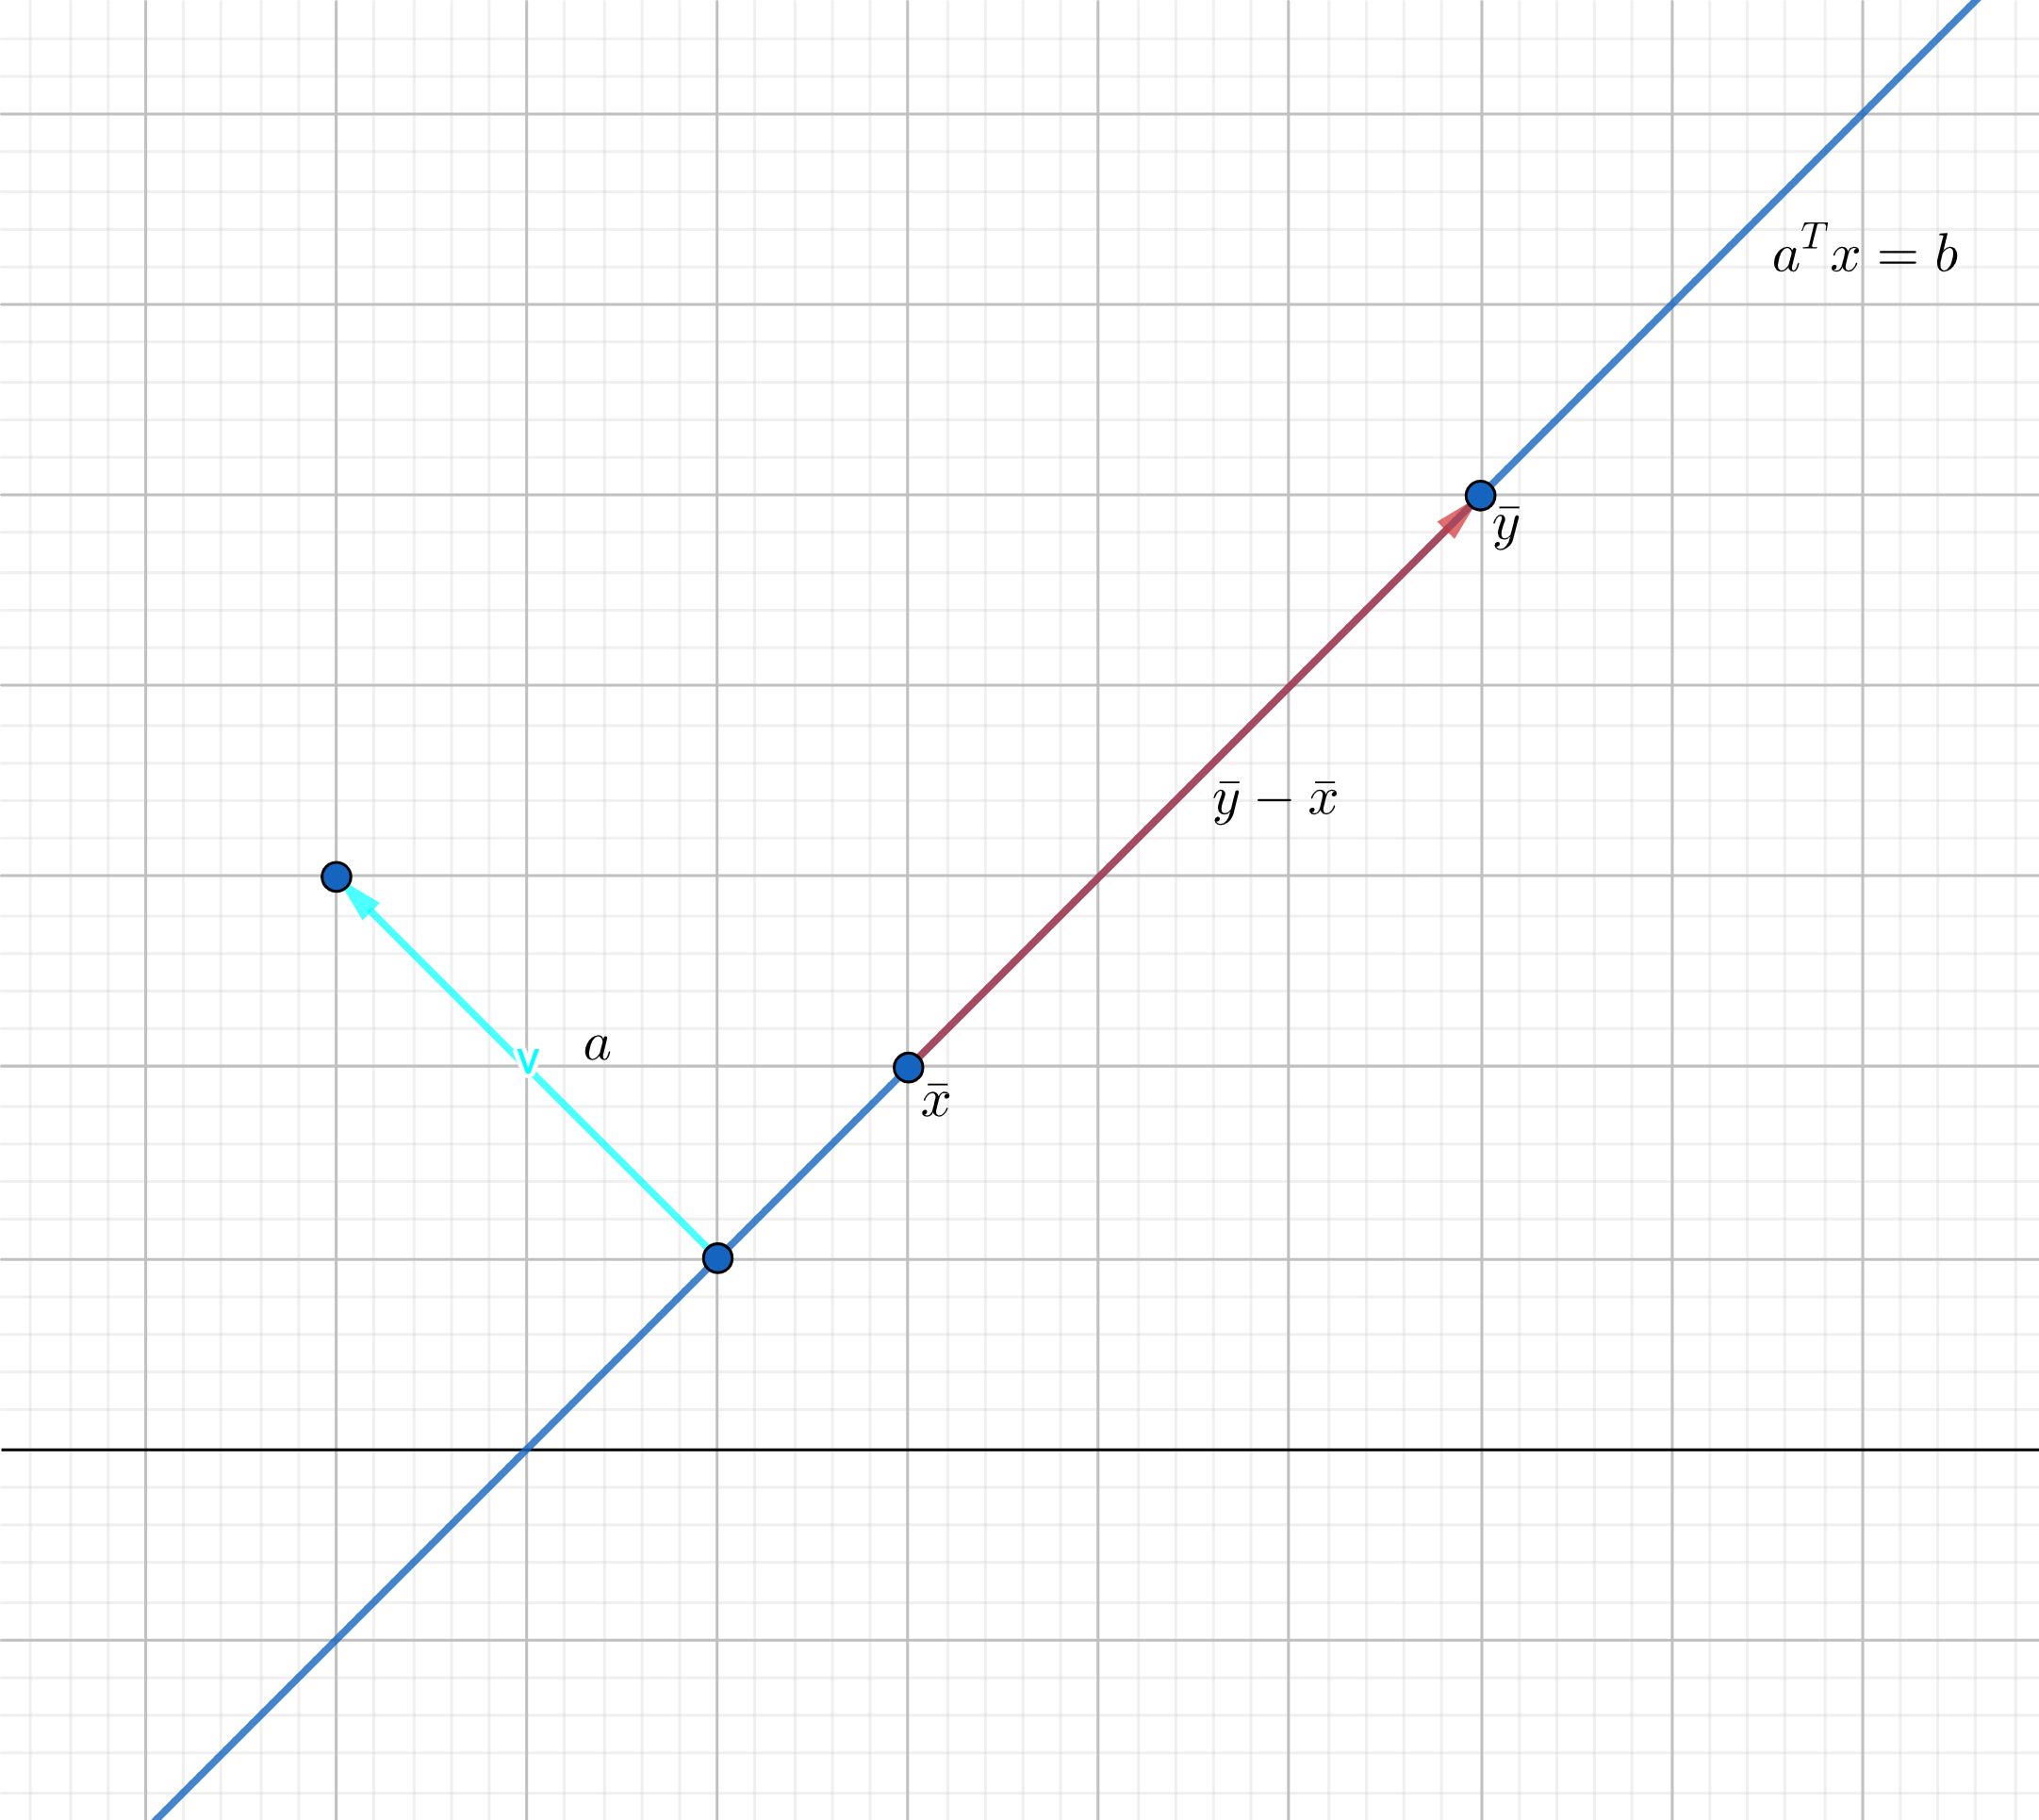
\includegraphics[scale=0.5]{angolirette.png}
\end{figure}

\noindent Questo ovviamente è valido per qualsiasi coppia di punti $\bar{x}$ e $\bar{y}$, quindi per ogni vettore che loro due formano.



\subsection{Rette, Semirette e Segmenti:} 

\paragraph{Retta:} Sia $\bar{x} \in \mathbb{R}^n$ un vettore (o punto, vettore e punto sono lo stesso oggetto), e sia d $\in \mathbb{R}^n$ (d di distanza) un altro vettore. Consideriamo un insieme parametrico di punti, con parametro $\lambda$: x($\lambda$) = $\bar{x}$ + $\lambda$ d. Al variare del parametro $\lambda \in \mathbb{R}$, $\bar{x}$ si muove sul grafico, disegnando una retta. Allora si ha:
\begin{equation*}
    R(\bar{x}, d) = \{x \in \mathbb{R}^n: x = \bar{x} + \lambda d, \lambda \in \mathbb{R}\}
\end{equation*}
è \textit{la retta passante per $\bar{x}$ e avente direzione d}

\paragraph{Semiretta:} Sia $\bar{x} \in \mathbb{R}^n$ un vettore, e sia d $\in \mathbb{R}^n$ un altro vettore. Definiamo l'insieme parametrico $x(\lambda) = \bar{x} + \lambda d$, ma stavolta $\lambda \in \mathbb{R}_+$. Allora:
\begin{equation*}
    S(\bar{x}, d) = \{x \in \mathbb{R}^n: x = \bar{x} + \lambda d, \lambda \in \mathbb{R}_+\}
\end{equation*}
è \textit{la semiretta passante per $\bar{x}$ e avente direzione d}. Nota che la semiretta è solo per $\lambda \in \mathbb{R}_+$, non è che se prendi $\lambda \in \mathbb{R}_-$ questa è la semiretta negativa e l'altra è la semiretta positiva. Tu prendi sempre $\lambda > 0$ e poi d decide il verso della retta, e quindi quale delle due semirette della retta devi prendere. Quindi la definizione \textit{generale} di semiretta è con $\lambda \in \mathbb{R}_+$, non era solo un esempio di semiretta, devi proprio sempre prendere $\lambda \in \mathbb{R}_+$, e poi se vuoi l'altra semiretta basta prendere d all'opposto, cioè se aveva componenti positive le prendi negative e hai l'altra semiretta.

\paragraph{Segmento:} Siano $\bar{x},\bar{y} \in \mathbb{R}^n$. Allora:
\begin{equation*}
    [\bar{x}, \bar{y}] = \{x \in \mathbb{R}^n: x = \lambda\bar{x} + (1 - \lambda)\bar{y}, \lambda \in [0,1]\}
\end{equation*}
Il segmento è una porzione limitata di retta. Questa definizione potrebbe richiamare la definizione di intervallo ma no non sono la stessa cosa perché l'intervallo è in $\mathbb{R}$ mentre questo è in un generico $\mathbb{R}^n$. Vediamo che si parla di un segmento perché per $\lambda = 0$ si ottiene $\bar{y}$, mentre per $\lambda = 1$ si ottiene $\bar{x}$. Per ogni valore tra 0 e 1 intermedi otteniamo i valori compresi tra gli estremi. Concludiamo dicendo che \textbf{Retta, Semiretta e Segmenti sono Insiemi Convessi}, che adesso definiremo. 

\subsection{Insieme Convesso:} Un insieme C $\subseteq \mathbb{R}^n$ è convesso quando, $\forall x,y \in C$, risulta [x,y] $\subseteq C$. Cioè quando, comunque presi due punti all'interno dell'insieme, il \textit{segmento} che li congiunge è contenuto \textit{interamente} nell'insieme stesso. 

\paragraph{Teorema:} L'intersezione di un numero finito qualsiasi di insiemi convessi è un insieme convesso. Dimostriamolo per due insiemi convessi. 

\subparagraph{Dimostrazione:} Prendiamo due insiemi convessi $C_1$ e $C_2$, e C = $C_1 \cap C_2$. Prendiamo x e y $\in$ C, ciò significa che x e y sono anche elementi sia di $C_1 e C_2$. Col fatto che questi sono convessi, il segmento che congiunge x e y è interamente contenuto in $C_1$ e anche in $C_2$. Quindi è interamente contenuto nell'intersezione tra i due, cioè C. Poiché il segmento che congiunge x e y è interamente contenuto in C, significa che C è convesso.



\subsection{Iperpiani e Semispazi:} 

\paragraph{Iperpiano:} Sia a $\in$ $\mathbb{R}^n$ e b $\in$ $\mathbb{R}$. Allora l'insieme:
\begin{equation*}
    H = \{x \in \mathbb{R}^n: a^{T}x = b\}
\end{equation*}
è un \textit{Iperpiano} in $\mathbb{R}^n$


\paragraph{Semispazi:} Sia a $\in \mathbb{R}^n$ e b $\in$ $\mathbb{R}$. Allora gli insiemi
\begin{equation*}
    S_{\geq} = \{x \in R^n: a^Tx \geq b\}
\end{equation*}
\begin{equation*}
    S_{\leq} = \{x \in R^n: a^Tx \leq b\}
\end{equation*}
Sono \textit{Semispazi}. Quindi un Iperpiano divide uno spazio in due Semispazi. Poniamoci questa domanda: un semispazio è un insieme convesso? Esempio:
$S_{\geq} = \{x \in R^n: a^Tx \geq b\}$ è convesso?

\subparagraph{Dimostrazione:} prendiamo
\begin{itemize}
    \item[I] $x \hspace{0.2cm} \text{t.c.} \hspace{0.2cm} a^Tx \geq b$ 
    \item[II] $y \hspace{0.2cm} \text{t.c.} \hspace{0.2cm} a^Ty \geq b$ 
\end{itemize}
Vogliamo far vedere che $\forall \lambda \in [0,1] \hspace{0.2cm} x(\lambda) = \lambda x + (1 - \lambda)y \in S_{\geq}$, giusto? Iniziamo moltiplicando (I) per $\lambda$ e (II) per $(1-\lambda)$, otteniamo:
\begin{itemize}
    \item[I] $\lambda a^Tx \geq \lambda b$ 
    \item[II] $(1-\lambda)a^Ty \geq (1-\lambda) b$ 
\end{itemize}
Adesso sommiamo termine a termine le due disuguaglianze:
\begin{equation*}
    \lambda a^Tx + (1-\lambda)a^Ty = a^Tx(\lambda) \geq \lambda b + (1-\lambda) b = b
\end{equation*} 
Da cui:
\begin{equation*}
    a^Tx(\lambda) \geq b
\end{equation*}
Quindi, poiché ci sono due punti x e y generici, all'interno del semispazio, e il loro segmento è interamente nello stesso semispazio, 
quindi il semispazio è un insieme convesso $S_{\geq}$ è un insieme convesso, e in generale \textit{tutti i semispazi sono insiemi convessi}.

\vspace{1cm}

\noindent Non solo, anche gli \textit{Iperpiano sono convessi}, dimostriamolo facilmente:
\begin{equation*}
    H = \{x \in R^n: a^Tx = b\}
\end{equation*}
Si tratta dell'intersezione dei due semispazi $S_{\leq} e S_{\geq}$, quindi essendo questi insiemi convessi, l'intersezione è convessa. Cioè tutti gli iperpiani sono convessi. Ovviamente questo risultato vale per $\mathbb{R}^n$ generico, quindi anche per $\mathbb{R}^2$ e $\mathbb{R}^3$: \textit{anche le rette e i piani sono insiemi convessi}. Bene, perché fare tutto questo? Perché questo adesso ci porta a dimsotrare che:

\paragraph{Teorema:} L'insieme ammissibile S di un problema di Programmazione Lineare (PL) è un insieme convesso. 

\subparagraph{Dimostrazione:} la regione ammissibile di un problema è data dall'intersezione di un numero finito di semispazi (vincoli con diseguaglianza) e iperpiani (vincoli con eguaglianze), quindi essendo sia i semispazi sia gli iperpiani convessi, la loro intersezione, cioè la regione ammissibile, è un insieme convesso.

\subparagraph{Nota:} Anche i due sottoinsiemi impropri di $\mathbb{R}^n$, cioè se stesso e l'insieme vuoto $\varnothing$, sono insiemi convessi. Anche un insieme composto da un solo punto è convesso. \textbf{Qualsiasi altro insieme composto da un numero FINITO di punti non è convesso}. Questo perché un segmento ha infiniti punti, quindi non può essere contenuto in un insieme con punti finiti.


\paragraph{Unione di insiemi convessi:} In generale l'unione di insiemi convessi non è convesso.


\section{Un problema di miscelazione:} Un'industria conserviera produce succhi di frutta (SF) mescolando polpa di frutta (P) e dolcificante (D). Il prodotto finale deve soddisfare alcuni requisiti sul contenuto di Vitamina C (V), Sali Minerali (S) e Zucchero (Z), che vediamo in questa tabella:
\begin{table}[h!]
    \centering
    \begin{tabular}{|c|c|c|c|c|}
    \hline
    & costo [\euro$_{cent}$/hg] & V [mg/hg] & S [mg/hg] & Z [g/hg]\\
    \hline
    P & 40 & 140 & 20 & 25\\
    \hline
    D & 60 & - & 10 & 50\\
    \hline
    SF & - & $\geq$ 70mg & $\geq$ 30mg & $\geq$ 75mg\\
    \hline
    \end{tabular}
\end{table}

\noindent Il nostro obiettivo è \textit{determinare le quantità ottime di P e D da miscelare}, per \textit{minimizzare i costi}. Come al solito, vogliamo matematicizzare questa situazione decisionale, e quindi dobbiamo porci la prima domanda che ci poniamo ogni volta in queste situazioni: \textit{cosa non conosciamo e vogliamo determinare?} Quelle saranno le nostre incognite. Noi non conosciamo le quantità di P e D da miscelare per ottenere abbastanza V,S e Z e spendere il meno possibile, quindi:
\begin{itemize}
    \item $x_1 \equiv$ q.tà [hg] di P da miscelare.
    \item $x_2 \equiv$ q.tà [hg] di D da miscelare.
\end{itemize}
In generale non c'è una regola per sapere quali sono le variabili, ma ci sono alcuni principi che ci aiutano:
\begin{itemize}
    \item Essere precisi nelle dimensioni delle quantità che usate.
    \item Vedere se riusciamo a esprimere attraverso le variabili ciò che serve esprimere, prima tra tutte la funzione obiettivo. In questo caso ci riusciamo. 
\end{itemize}
Bene, allora esprimiamola sta funzione obiettivo:
\begin{equation*}
    f(x) = Costo tot. = 40x_1 + 60x_2 
\end{equation*}
Bene, questa ricordiamoci che va minimizzata. Ora passiamo ai vincoli:
\begin{equation*}
    Vitamine tot. = 140 \frac{mg}{hg} \cdot x_1 hg  + 0\frac{mg}{hg} \cdot x_2 = 140x_1 mg \geq 70 mg
\end{equation*}
\begin{equation*}
    Sali tot. = 20x_1 + 10x_2 \geq 30
\end{equation*}
\begin{equation*}
    Zucchero tot. = 25x_1 + 50x_2 \geq 75
\end{equation*}
Manca una sempreverde condizione, che \textit{dobbiamo sempre ricordarci quando abbiamo a che fare con delle quantità}: \underline{esse non possono essere negative}.
\begin{equation*}
    x_1 \geq 0 
\end{equation*}
\begin{equation*}
    x_2 \geq 0 
\end{equation*}
Notiamo che $x_1 \geq 0$ è ridondante, poiché dalla prima condizione vediamo che $x_1 \geq \frac{1}{2}$. Disegnamo la zona ammissibile, nello stesso modo in cui abbiamo fatto la prima volta, e ci esce fuori:
\vspace{1cm}

\begin{tikzpicture}
  \begin{axis}[
    axis lines=middle,
    xmin=0, xmax=3,ymin=0,ymax=3
  ]
  \addplot[thin,white, samples=300, domain=0:3, name path=A] {3}; %linea invisibile per far colorare pgfplots
  \addplot[very thick,yellow!70!red, samples=300, domain=0:3, name path=B] {(30 - 20*x)/10}; %passa per (0,3) e (3/2,0)
  \addplot[very thick,red!90!teal, samples=300, domain=0:3, name path=C] {(75-25*x)/50}; %passa per (0,3/5) e (3, 0)
  \addplot[very thick,blue!90!teal, samples=300, domain=0:3, name path=D] {0}; 
  \addplot[gray!30] fill between[of=A and B, soft clip={domain=1/2:1}];
  \addplot[gray!30] fill between[of=A and C,soft clip={domain=1:3}];
  \end{axis}
  \draw[green] (1.146,0) -- (1.145,5.7); % per disegnare la retta x = 1/2
\end{tikzpicture}

\noindent Notare che questa volta, a differenza della prima, la zona ammissibile è illimitata. Bene, ora passiamo alla funzione obiettivo. La funzione obiettivo $40x_1 + 60x_2 = k$ descrive un \textit{fascio di rette parallele}. Prendendo la retta di questo fascio $40x_1+60x_2 = 0$, vediamo che nessun punto di questa retta passa per la zona ammissibile. Questo perché mi sto domandando se esistono produzioni ammissibili, cioè coppie ($x_1,x_2$) che mi permettano di avere Costo tot. = 0 e rispettare i vincoli di V, S e Z totale, e ovviamente questo non è possibile. Proviamone un'altra, per esempio la retta del fascio che passa per il punto (3,0) intersezione della retta con l'asse x. Sostituendo $x_1 = 3$ e $x_2 = 0$ nell'equazione $40x_1 + 60x_1$ = k troviamo k = 120, cioè questa è la retta dei punti che mi fanno guadagnare 120. Ma vedo che posso trovare anche di meglio, spostandola più in basso (ricordiamo che stiamo cercando di minimizzare la funzione). Provando le altre intersezioni rimaste (in zona ammissibile) vediamo che il miglior punto è (1,1), dove k = 100, e spendiamo il minimo possibile. Se io volessi spendere meno di 100 devo considerare rette sotto la retta del fascio per cui ottengo 100, ma nessuna di queste passa per la zona ammissibile.

\subparagraph{Nota (penso che dopo il professore ce lo dirà formalmente):} \textit{i punti di ottimizzazione} (sia di massimizzazione che di minimizzazione) si trovano SEMPRE in un punto di intersezione tra due rette che formano la zona ammissibile, quindi cerca in quei punti se vuoi trovare il valore ottimo!


\subparagraph{Domanda di un alunno:} Professore ma se il fascio di rette generato dalla funzione obiettivo è parallelo a un vincolo, avremmo un insieme di punti come soluzione? Ha risposto di sì, ma tanto a te sempre l'intersezione ti interesserebbe, anche in quel caso, perché anche in quel caso puoi trovare un punto intersezione tra le rette.







\subsection{Altro esempio:}
\begin{equation*}
    S = \{(x,y) \in R^2, x^2 + y^2 \geq 1, x + y \geq 2\}
\end{equation*}
Vediamo che S, essendo l'intersezione tra l'area al di fuori del cerchio e un sottoinsieme di quest'area (cioè  $x + y \geq 2$), è proprio uguale a quest'ultima. Essendo quest'ultima convessa, anche S è convesso. Notare che il fatto che un'area sia contenuta in un'altra, porta l'equazione di quest'ultima ad essere ridondante, come in questo caso è l'equazione del cerchio. Bene, ora classifichiamo S:
\begin{itemize}
    \item S è un problema di ottimizzazione? Sì, perché può essere scritto nella forma:
    \begin{equation*}
        min f(x)
    \end{equation*}
    \begin{equation*}
        x \in S = \{(x,y) \in R^2, x^2 + y^2 \geq 1, x + y \geq 2\}
    \end{equation*}
    \item S è un problema di Programmazione Matematica? Sì, perché esso è definito solo da disuguaglianze
    \item S è un problema di PL? No, perché c'è un'equazione non lineare. 
\end{itemize}
Quindi questo è un problema di PNL. Notare che \textit{non importa che l'equazione che rende il problema non lineare sia ridondante, non possiamo pensare di non considerarla} solo perché è ridondante! Comunque non è lineare, anche se se la eq. ridondante venisse eliminata il problema diventerebbe PL, perché in questo caso staremo definendo un'altra S e quindi un altro problema.


\newpage

\section{Esercizi:} 

\paragraph{1:} Una industria è specializzata nella fabbricazione di un prodotto per il fai-da-te in due qualità differenti standard e deluxe. Ciascuna unità di prodotto richiede (tra le altre) una fase di smerigliatura ed una di pulitura. In tabella sono riportati i tempi di lavorazione delle due fasi in ore (per unità di prodotto); i prezzi di vendita in e (per unità di prodotto)
\begin{table}[h!]
    \centering
    \begin{tabular}{|c|c|c|}
    & standard &  deluxe \\
    smerigliatura [h/u] & 4 & 3\\
    pulitura [h/u] & 2 & 5\\
    prezzo [\euro/u] & 10 & 15
    \end{tabular}
\end{table}
Le macchine adibite ai due processi di smerigliatura e pulitura lavora per, risp., 80 e 60 ore per settimana. Scrivere un problema di PL che consenta di determinare il piano ottimo di produzione settimanale (ipotizzando che tutto ciò che viene prodotto sia venduto).
\begin{itemize}
    \item Individuare le variabili di decisione specicandone precisamente l'unità di misura
    \item Scrivere la funzione che si vuole massimizzare o minimizzare specicandone precisamente l'unità di misura
    \item Scrive i vincoli che limitano le scelte possibili specicandone precisamente l'unità di misura
\end{itemize}


\subparagraph{Risposta:} 

\


\begin{figure}[h!]
    \centering
    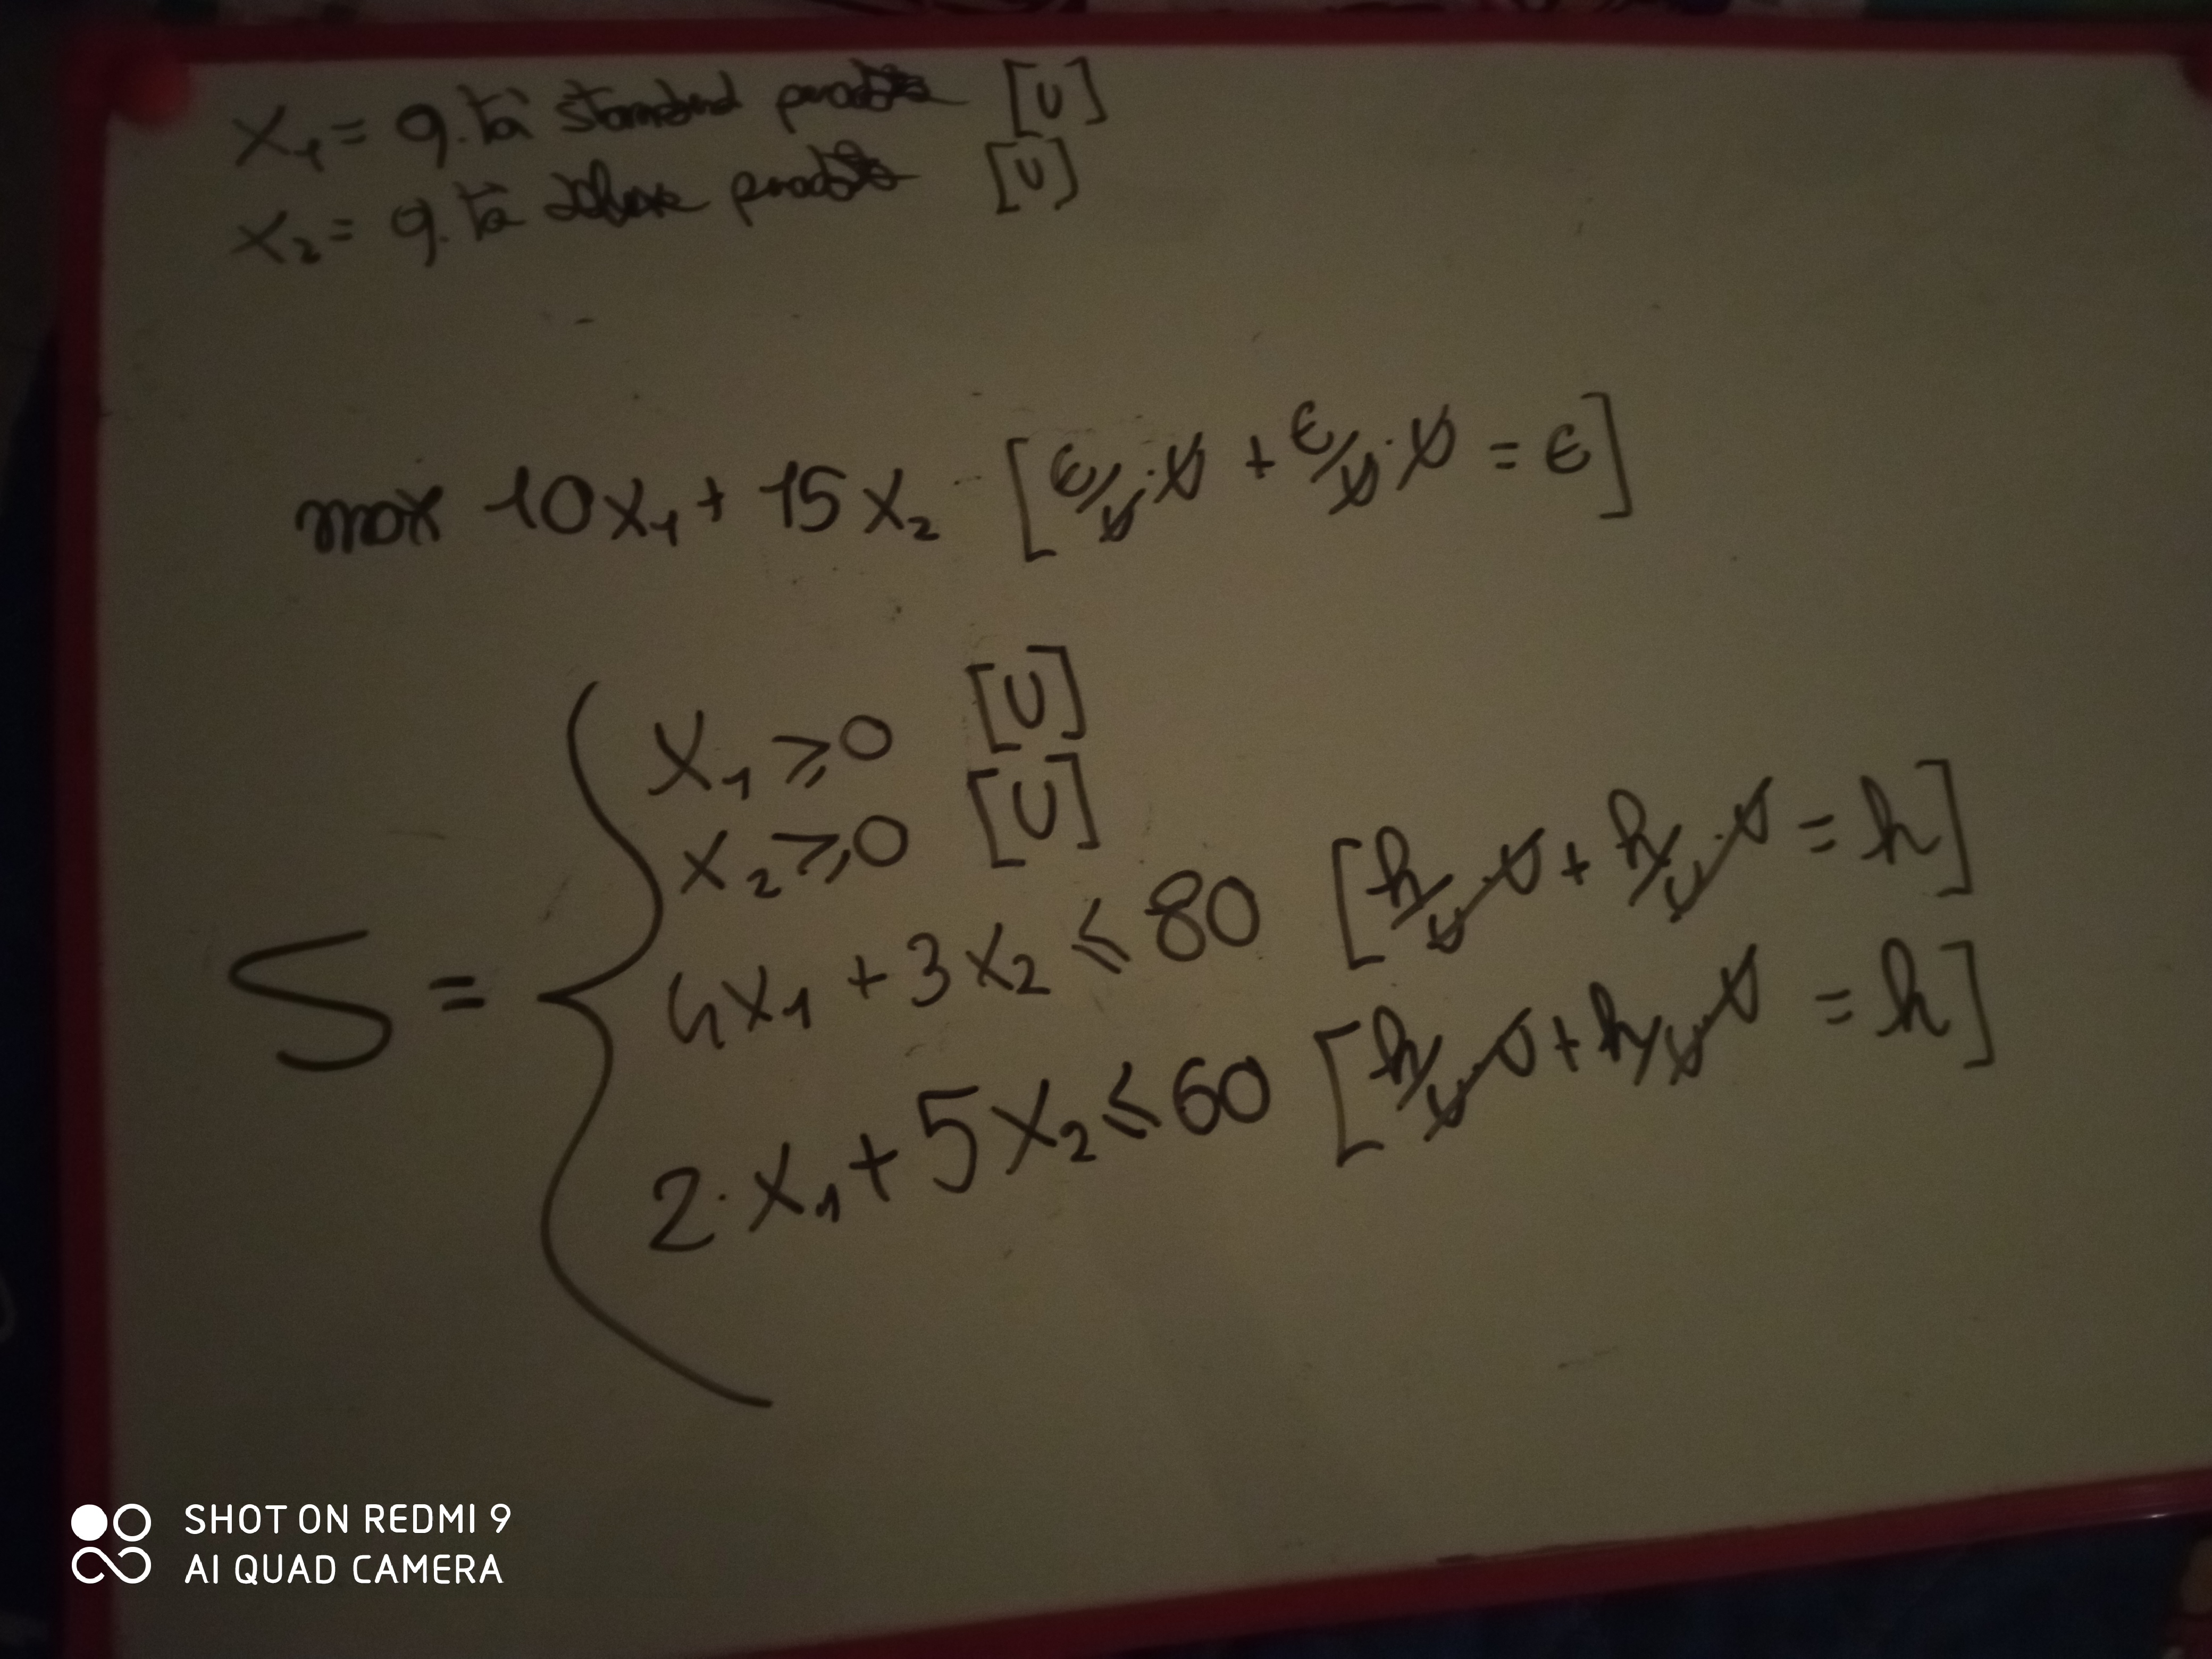
\includegraphics[scale=0.05]{esercizio2.jpg}
\end{figure}
ATTENZIONE!!! Le variabili di decisione $x_1$ e $x_2$ non sono unità MA unità per settimana. In conseguenza di ciò, i vincoli sono in ore per sett. e la f.ob. in euro per sett. \textcolor{red}{CORREGGERE!!!!!!!!!}

\paragraph{2.} Dato il seguente sistema di disuguaglianze lineari (che rappresenta la regione ammissibile di un ipotetico problema di PL)
\begin{equation*}
    \begin{cases}
        \text{$x1 + 3x2 + 2x3 \leq 3$}\\
        \text{$4x1 + x2 + x3 \geq 5$}\\
        \text{$x3 \leq 1$}\\
        \text{$x1 \geq 0$}\\
        \text{$x3 \geq 0$}
    \end{cases}
\end{equation*}
\begin{itemize}
    \item Quanti vincoli sono attivi in (0, 1, 0)?
    \item Quanti vincoli sono violati in (0, 1, 0)? Il punto (0, 1, 0) è ammissibile?
    \item Quanti vincoli sono attivi in (1, 0, 1)? Il punto (1, 0, 1) è ammissibile?
    \item Quanti vincoli sono attivi in (1, 0, 1)?
    \item Il punto (1, 0, 1) è ammissibile?
\end{itemize}

\subparagraph{Risposta:} 

\

\begin{figure}[h!]
    \centering
    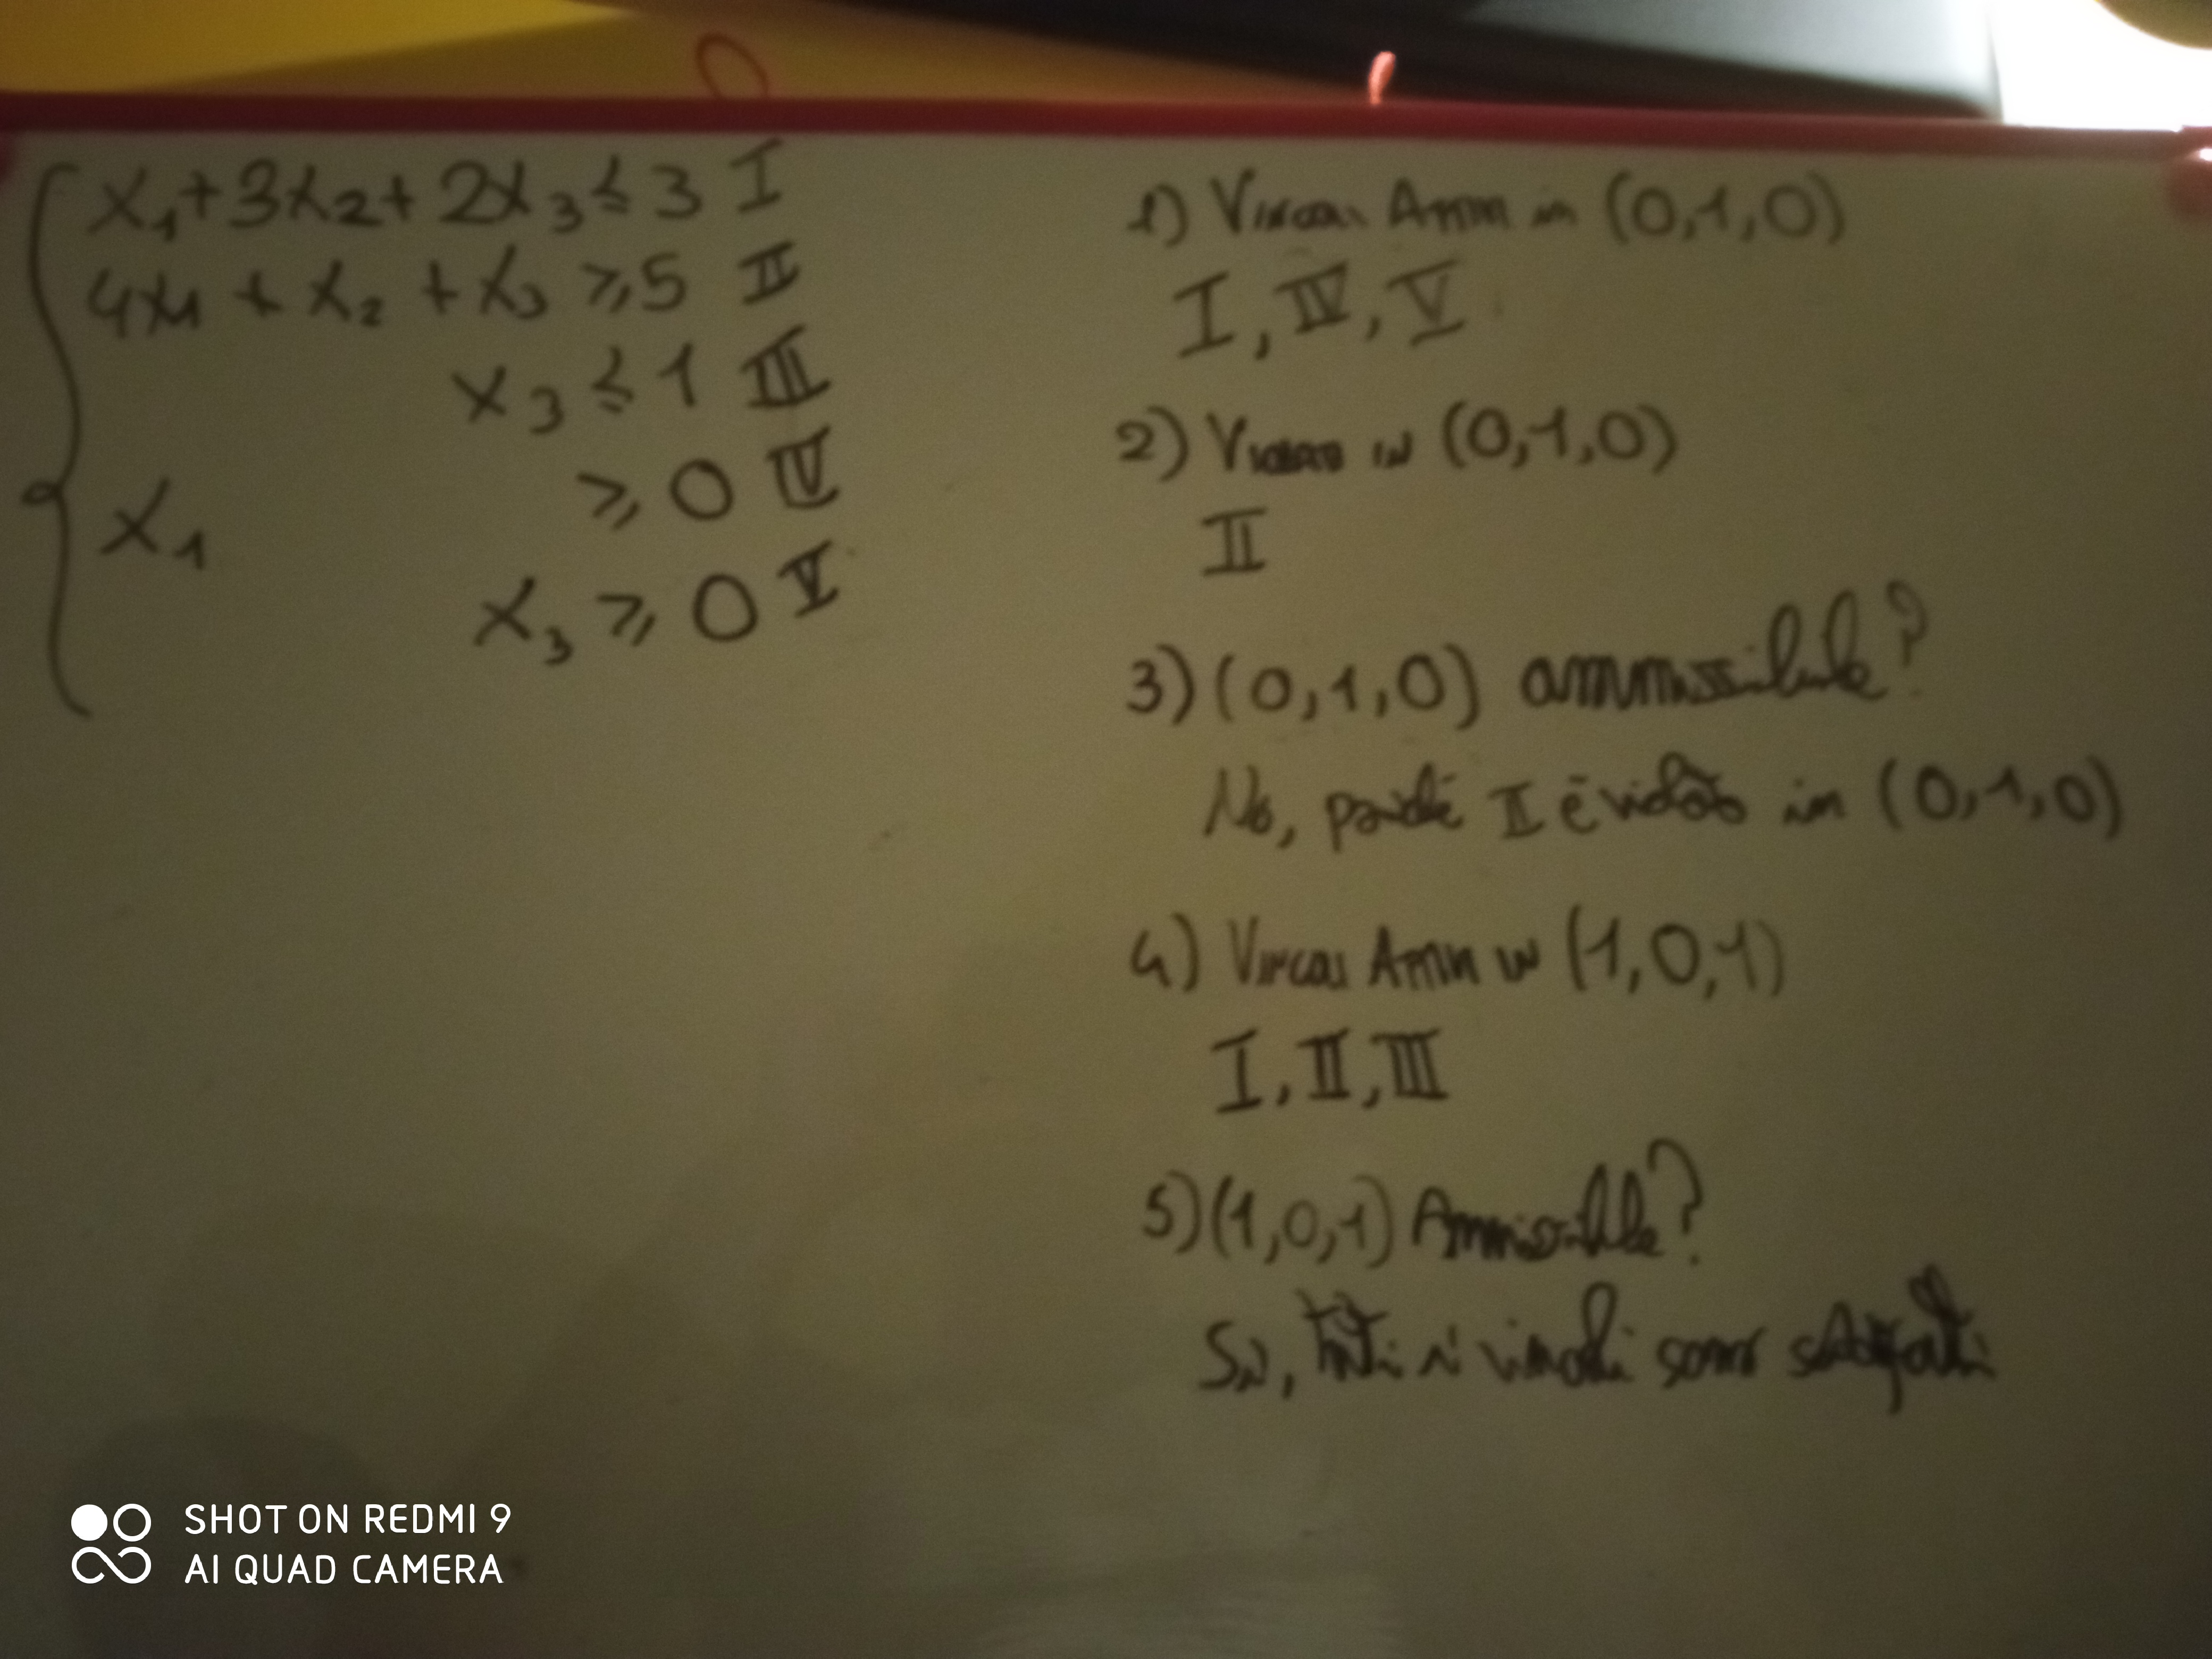
\includegraphics[scale=0.05]{esercizio1.jpg}
\end{figure}
























